\documentclass[a4paper,12pt]{article}

\usepackage[utf8]{inputenc}
\usepackage[margin=1.0in]{geometry}
\usepackage{graphicx}

\title{Examining Network Hyperparameters for \\ Thermopile Imaging Recognition}
\author{Robert Scott}
\date{February 26th, 2021}

\begin{document}

\maketitle

\begin{abstract}
This paper examines various hyperparameters as used in training multilayer perceptrons. It is a comparative study between two neural network training architectures: a network trained using backpropagation and a network trained using swarm intelligence.
\end{abstract}

\section{Introduction}
A thermopile camera is an infrared sensor which captures imaging data from the environment. It works similarly to a typical digital camera but instead focuses on capturing only the infrared end of the light spectrum. Infrared light is invisible to the human eye and sensing infrared is analogous to sensing temperature. Of note is that these sensors are well suited to identifying the presence of humans or other animals because the body temperature is typically greater than its surroundings.

\section{Problem Definition}
The usefulness of a thermopile camera, however, remains limited without adequate means to identify subjects it captures. The human brain is adept at picking out patterns, especially faces, from images, but the data a thermopile camera provides may not be easily machine readable.

\begin{figure}[h!]
\centering
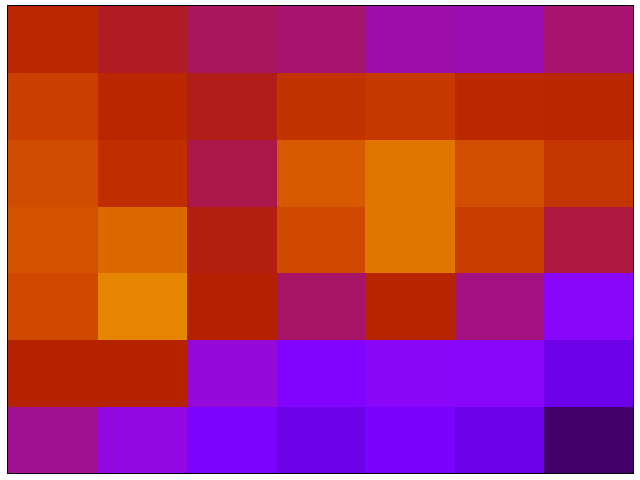
\includegraphics[scale=0.35]{images/heat1.png}
\caption{An 8x8 resolution thermopile capture, two subjects}
\label{fig:heatmap1}
\end{figure}

\pagebreak

In the above figure, an 8x8 resolution capture from a thermopile sensor is shown. Each pixel in this image corresponds to a certain color denoting the intensity of temperature, with more red appearing hotter and more blue appearing colder.

It may or may not be apparent that in this image exists two human faces, as denoted by two hotspots. In this example image, there is relatively clear delineation between subjects and background which makes it simple to see.

\begin{figure}[h!]
\centering
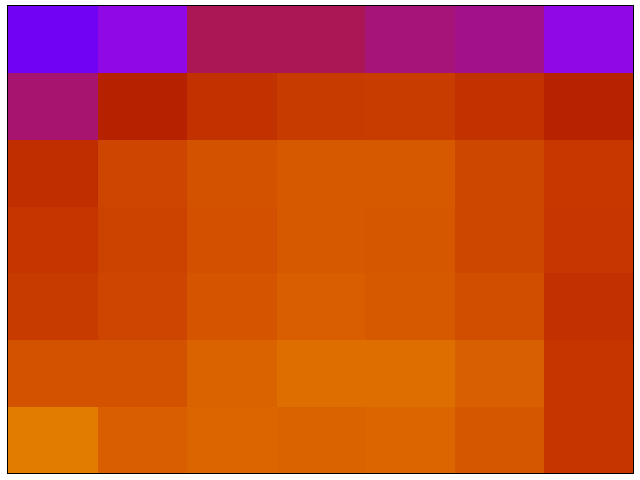
\includegraphics[scale=0.35]{images/heat4.png}
\caption{An 8x8 resolution thermopile capture, no subject}
\label{fig:heatmap4}
\end{figure}

However, for some captures such as the above figure, it can be difficult to discern subjects or the absence thereof. But, what may be difficult for a human to understand may be made easier by use of machine learning techniques such as neural networks.

\section{Neural Networks}

A neural network is a biologically inspired tool under the broader class of machine learning algorithms [3]. It consists of a sequence of layers, themselves consisting of interconnected nodes---called neurons. The biological analogy is the brain, where this technique of machine learning takes its namesake. Neural networks can be used for many tasks, of note is the classical usage scenario of classification [5]: given an input, identify which class of objects that input belongs to.

\begin{figure}[h!]
\centering
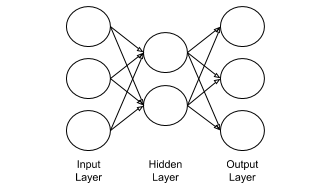
\includegraphics[scale=0.65]{images/network-diagram.png}
\caption{A 3-2-3 network}
\label{fig:network_diagram}
\end{figure}

Neural networks on the surface can be obtuse: they're mathematically robust but conceptually abstract, and are often considered black-boxes. While the inputs and outputs may be known, the inner workings can be difficult to discern.

\pagebreak

As mentioned, neural networks are organized in layers, where each layer is connected to the prior and subsequent layer via its neurons. Typically, a network consists of an input layer---which acts as data intake---one or more hidden layers, and then finally a lone output layer---which acts as classifier.

In \textbf{figure 3} above, a network topology is given, showing three input neurons, a lone hidden layer consisting of two neurons, and three output neurons. What this signifies is the network intakes three-dimensional data and will attempt to classify the data into one of three distinct classifications.

Consider a scenario of identifying the vehicle type of an object given three characters, where available classifications are sedan, coupe, or hatchback. The characteristics could be length of vehicle, how many doors, and truck space. This is one example where this type of network might exist.

A neural network also contains synaptic weights between layers by way of neural connections. While numerically defined, they describe how strong a signal between neurons is.

\begin{figure}[h!]
\centering
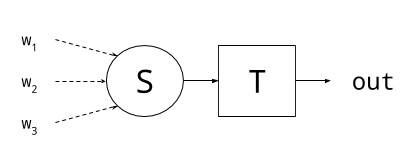
\includegraphics[scale=0.7]{images/neuron-diagram.png}
\caption{A neuron}
\label{fig:neuron_diagram}
\end{figure}

In the above figure is a neuron comprising of many parts; from left to right: some synaptic weights, a summing function, transfer function, and an output. The neuron accepts some inputs, multiplied by the synaptic weights, these values are them summed, and sent to a transfer function to be activated. This function determines to what degree a neuron "fires" based on the summation, which is some ratio if its inputs (rationed by the varying weights). This "firing" corresponds to how much the intake data is important for the current training example [3].

A network is fed training examples which flow through the network from input layer to output layer in a process called \textit{feedforward}. Then, by some training mechanism, will adjust the synaptic weights such that the signals received at the output layer more closely resemble the correct known classification if the input data [3]. This entire process is a type of \textit{supervised learning}, where classifications are known a priori for some set of training examples and given enough of them, the network will learn to generalize for novel inputs.

\pagebreak

\section{Network Architectures}

There are numerous ways to train a neural network: two of which being a gradient-based training method, and a metaheuristic-based training method.

\subsection{Backpropagation}

Typically, the most popular approach to training a neural network is using \textit{backpropagation}, which is a gradient-based training strategy which relies on the existence of an error gradient between an anticipated output target value and an actual output [3].

When an example is fed into the network, an error is found and needs to be fed "backwards" through the network to correct weights: this is backpropagation.

However, where backpropagation suffers is in the possibility of exploding or vanishing gradients [2], where the error gradient can become infinitesimally small or extremely large. Not only this which can lead to stagnation or early convergence to a suboptimal solution. Not only this, but using backpropagation requires the classification problem to be linearly differentiable which is not always the case for every problem.

\subsection{Particle Swarm Optimization}

An alternative is to use a method of training which does not rely on differential calculus or gradients, such as metaheuristics. A metaheuristic is a local-global search algorithm which aims to minimize a loss function---not unlike backpropagation---and it is a method which abstains from differential calculus or error gradients [3].

One such example of a metaheuristic is \textit{particle swarm optimization}, which takes cues from the social behavior of flocking birds. Instead of reinforcement learning through continual feeding of training examples, particle swarm optimization instead treats the network as a multidimensional optimization problem, taking control of synaptic weights directly by creating a swarm of "particles" corresponding to weights and readjusting their position based on arithmetic and some parameters which control their movement [1].

\section{Experimental Setup}

Implemented were a backpropagation trained feedforward network (\textbf{BP-NN}) and a particle swarm trained feedforward network (\textbf{PSO-NN}) in an attempt to analyze the efficacy of training when varying different network hyperparameters. A training suite was developed to concurrently train multiple networks and record data relevant to accuracy in classification.

In order to analyze the efficacy of network training, several network hyperparameters must be tested. Additionally, results collection needs to be explained.

Intake data is in the form of tuples with 64 attributes and a lone classification---of which there are 9 distinct possibilities. The data corresponds to thermopile images of a varying number of subjects (one, two, three subjects and the absence of a subject) and distances from sensor (one and three feet). Images can be taken indoors or outdoors. From the entire data set, $70\%$ of data is used for training the network, and the remaining $30\%$ of data is used to test the network for \textit{holdout training}.

\pagebreak

\begin{figure}[h!]
\centering
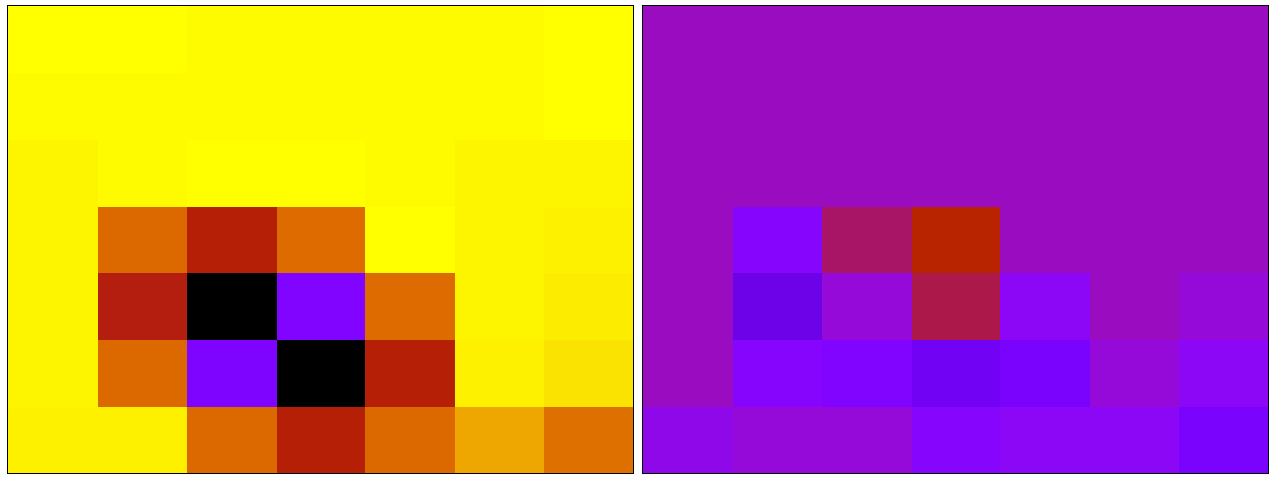
\includegraphics[scale=0.35]{images/heat2.png}
\caption{An example capture of outdoor data before and after thresholding}
\label{fig:heat2}
\end{figure}

This data is first prethresholded to account for extremely hot images: any attribute over 1000 is divided by 100, filtering out all values on the extreme end. Then, data is normalized, centering all data around the origin and adjusting data such that attributes are all of similar magnitudes. These two preprocessing steps are done to ensure better delineation between subjects and backgrounds. See \textbf{figure 5} for an example.

There are twelve tests for backpropagation and fourteen tests for particle swarms. Each test is performed thirty times with the worst seven runs of each being discarded. Since networks are stochastic, there is a chance of failure to converge entirely, and removing this potential ensures runs are indicative of correct and complete data.

For backpropagation, three parameters are examined: hidden layer size, which denotes how large the lone hidden layer is and concerns network topology. A larger hidden layer may be able to extricate the nuances of data better but training speed---not only in execution speed but also convergence speed---may suffer.

There are also learning and momentum rates [3, 4]. When an example is fed into the network, the error is found in the output layer and is backpropagated back into the previous layers: how much of this error is determined by the learning rate, or how much of this error should be considered when adjusting weights in the backwards pass of backpropagation.

Momentum rate is similar, but considers the prior example's error to exert a "force" onto the current example [4]. When error is found for one example, it is stored as a temporal error delta and re-used in the subsequent example, imparting some momentum. To what degree this momentum is applied is governed by the momentum rate.

\begin{table}[h!]
\centering
\begin{tabular}{c|c|c|c|}
\cline{2-4}
 & \textbf{Hidden Layer Size} & \textbf{Learning Rate} & \textbf{Momentum Rate} \\ \hline
\multicolumn{1}{|c|}{Test 1} & 5 & 0.001 & 0.001 \\ \hline
\multicolumn{1}{|c|}{Test 2} & 10 & 0.010 & 0.010 \\ \hline
\multicolumn{1}{|c|}{Test 3} & 15 & 0.100 & 0.100 \\ \hline
\multicolumn{1}{|c|}{Test 4} & 20 & 1.000 & 1.000 \\ \hline
\end{tabular}
\caption{BP-NN test parameters}
\label{Tab:bp-nn-tests}
\end{table}

In the above table, the different tests for backpropagation training are enumerated with their test number and specific parameters.

\pagebreak

For particle swarms, three parameters are examined as well: hidden layer size---which is an identical test to the one for backpropagation---and swarm size, which is the number of particles within a swarm, where generally more is slower but more accurate.

The final parameter is a set of three values: inertial weight, which considers how resistant to change in position a particle has; the cognitive coefficient, which considers how much a particle's personal best position and the swarm's best position influences its movement.

\begin{table}[h!]
\centering
\begin{tabular}{c|c|c|c|}
\cline{2-4}
 & \textbf{Hidden Layer Size} & \textbf{Swarm Size} & \textbf{Swarm Parameters} \\ \hline
\multicolumn{1}{|c|}{Test 1} & 5 & 10 & $\omega = 0.25, c_1 = 1.35, c_2 = 1.05$ \\ \hline
\multicolumn{1}{|c|}{Test 2} & 10 & 25 & $\omega = 0.35, c_1 = 1.45, c_2 = 1.15$ \\ \hline
\multicolumn{1}{|c|}{Test 3} & 15 & 50 & $\omega = 0.45, c_1 = 1.55, c_2 = 1.25$ \\ \hline
\multicolumn{1}{|c|}{Test 4} & 20 & 75 & $\omega = 0.55, c_1 = 1.65, c_2 = 1.35$ \\ \hline
\multicolumn{1}{|c|}{Test 5} & N/A & 100 & $\omega = 0.65, c_1 = 1.75, c_2 = 1.45$ \\ \hline
\end{tabular}
\caption{PSO-NN test parameters}
\label{Tab:pso-nn-tests}
\end{table}

In the above table, the different tests for particle swarm training are enumerated likewise.

The results of the network is determined by finding the \textit{mean squared error} (\textbf{MSE}) of the output layer after each epoch of training. The MSE is a measure of how much error exists within the output layer, where a lower MSE correlates to better classification accuracy.

\begin{figure}[h!]
\centering
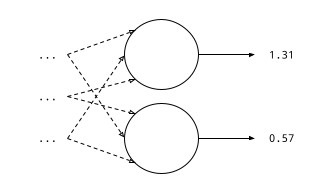
\includegraphics[scale=0.85]{images/classification-threshold.png}
\caption{An example output layer with outputs}
\label{fig:classification}
\end{figure}

The network effectively outputs a set of probabilities that a training example belongs to a specific classification. In the above figure, two output neurons exist with outputs of $1.31$ and $0.57$ respectively. In this example, the uppermost output neuron has fired more, which means there is more confidence in the classification belonging to this neuron. In other words, the input data correlates to the first classification of the network. Whichever output neuron fires the most is considered the network's guess at the classification.

Two statistical tests are utilized to determine if experimental results are significant. \textit{One-Way ANOVA}, which examines the variances and means of sample populations to determine whether there is stochastic dominance between any sample set and tests the null hypothesis, which suggests that all samples are from the same broader population (in other words, there is no significant difference between samples). 

\textit{Tukey's range test} is a similar test which is used to test pairwise variances and means between sample populations. How it differs from the One-Way ANOVA test is if an ANOVA test discovers some stochastic dominance between samples, Tukey's range test can determine where the dominance comes from.

These two tests are used to analyze the MSE per epoch data to determine if one set of parameters is preferable to another and will make an attempt to find the best parameters to use in training.

\section{Experimental Results \& Discussion}

Using the automated training suite, tests are performed autonomously then concatenated and formatted in a way that allows for plotting the MSE over many epochs. 25 epochs were chosen as it best visualized in plots and was sufficient enough to ascertain whether a network would converge or stagnate.

\subsection{BP-NN Hidden Layer Test}

The comparison between hidden layer size for backpropagation training illustrates the below plot:

\begin{figure}[h!]
\centering
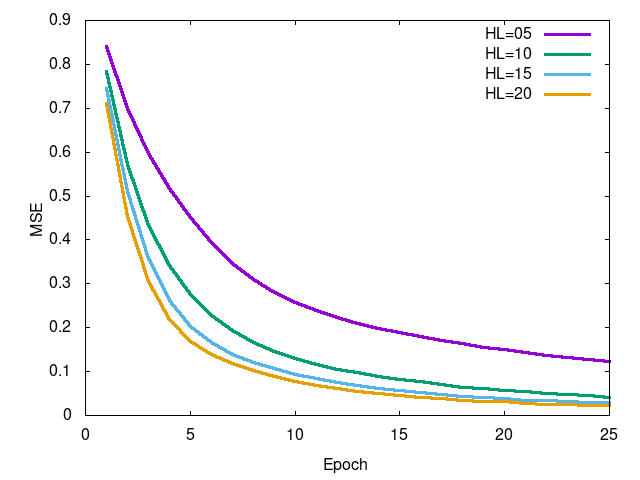
\includegraphics[scale=0.60]{images/bp-hl-plot.png}
\caption{Collected results for BP-NN Hidden Layer test}
\label{fig:bp-nn-hl}
\end{figure}

While every curve in this plot converged to a termination condition of $MSE \leq 0.2$, visually they are distinct with some curves approaching convergence quicker than others.

On performing an ANOVA test, a $p$ value of $p = 0.004367$ is found, alongside an F-score of $F = 4.66388$ ($F \geq 1.0$ suggests perfect test reliability), less than the null hypothesis $H_0 : p \geq 0.05$. Accepting the null hypothesis means there is no stochastic dominance between samples and it can be concluded that each sample is taken from the same population. However, since $p < 0.05$, the null hypothesis is rejected suggesting there is enough variance between tests that there is one or more candidates that perform better or worse than the others.

\pagebreak

Since there is evidence of stochastic dominance, Tukey's range test is performed to compare pairwise means between samples. This test finds that of the tests, pairs involving five hidden layers (HL=05) show significant difference, suggesting that this test is an outlier.

Removing this sample from the set of tests and then performing another ANOVA tests leads to a $p$ value of $p = 0.524475$, which means the null hypothesis---that there is no statistically significant difference between samples---is accepted.

The results from these statistical tests and from the data suggest that between $10$, $15$, and $20$ neurons in the hidden layer, there is no significant advantage in choosing one over the other. For this reason, a hidden layer size of $10$ is chosen as preferable as it will result in expedient training and convergence [3].

\subsection{BP-NN Learning Rate Test}

On comparing the learning rate parameter for backpropagation, the below plot is generated:

\begin{figure}[h!]
\centering
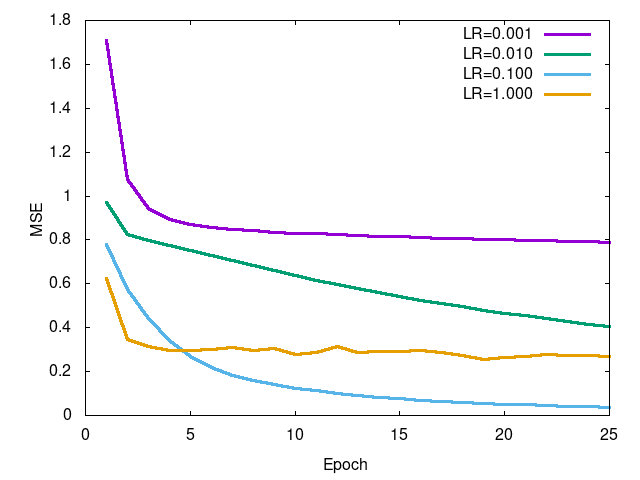
\includegraphics[scale=0.60]{images/bp-lr-plot.png}
\caption{Collected results for BP-NN Learning Rate test}
\label{fig:bp-nn-lr}
\end{figure}

Unlike the previous test, only one learning rate converged to the termination condition and the others either stagnated or were too slow to converge.

On performing an ANOVA test, a $p$ value of $p < 0.00001$ is found, suggesting significance in difference of variances and means between samples: the null hypothesis is rejected as there is evidence of significant difference between learning rates. The F-score for this test was $F = 103.85039$ suggesting strongly the test is confident.

To verify, Tukey's range test is performed on pairwise combinations of samples and it is found that every pair has significant difference of means. This test concludes that there is advantage to choosing one learning rate over another but is inconclusive on which learning rate is an outlier.

Since Tukey's test showed significance in choosing one sample but cannot discern which to use or avoid, the sample with the smallest mean is chosen: a learning rate of $0.100$.

\pagebreak

As to why some learning rate choices converged slowly or did not converge, it is either the learning rate was too high, overshooting a minima or getting trapped in a local minima [3]. The learning rate affects how much weights are corrected in the backpropagation step, and it stands to reason that too little will not learn (or learn as quickly) and too much will overcorrect too much, as evidenced in the above plot.

\subsection{BP-NN Momentum Rate Test}

The momentum rate test for backpropagation produces the below plot:

\begin{figure}[h!]
\centering
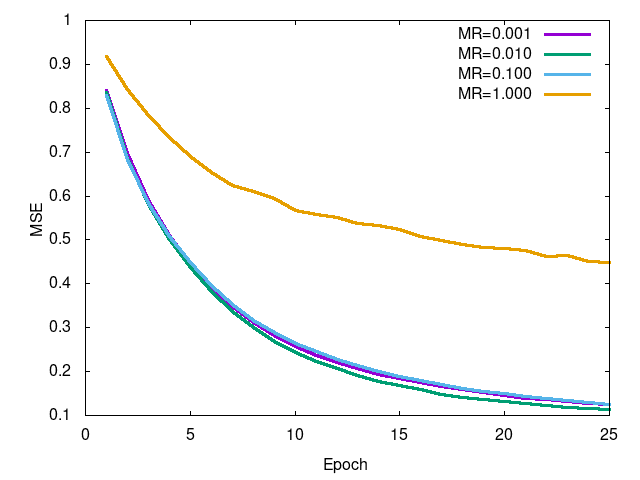
\includegraphics[scale=0.60]{images/bp-mr-plot.png}
\caption{Collected results for BP-NN Momentum Rate test}
\label{fig:bp-nn-mr}
\end{figure}

If not obvious visually, three tests have roughly equal performance where one test is an outlier with a much slower convergence.

An ANOVA test produces a $p$ value of $p < 0.0001$ and an F-score of $F = 17.30395$. These results suggest the null hypothesis is rejected with strong confidence in the test being accurate. This means there is significance in choosing (or not choosing) at least one parameter over another.

Tukey's range test is again used and it is found through analysis of pairwise mean comparisons between samples that a momentum rate of $1.000$ is an outlier with a much higher mean than the other samples.

The other momentum rates do not suggest significant difference of means as proven by performing another ANOVA test with the MR=1.000 sample removed.

This suggests there is no difference in choosing a momentum rate between $0.001$, $0.010$, or $0.100$. There is no benefit to choosing a smaller momentum rate in this instance because momentum rate will (generally) not impact speed of execution [4], so any momentum rate from those three tests is adequate.

As to why a momentum rate of $1.000$ did not converge, it is not dissimilar for the reason a learning rate of $1.000$ did not converge: the momentum has exerted too much force on weight correction that weights were overcorrected or minima were overshot.

\pagebreak

\subsection{PSO-NN Hidden Layer Test}

On testing hidden layer size for the particle swarm trained network, the below plot is made:

\begin{figure}[h!]
\centering
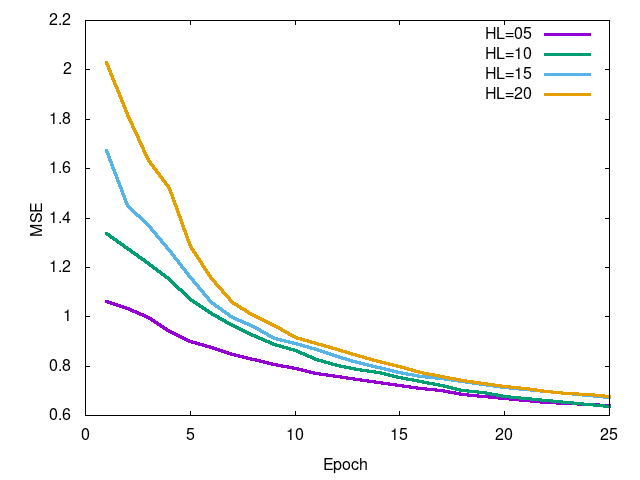
\includegraphics[scale=0.60]{images/pso-hl-plot.png}
\caption{Collected results for PSO-NN Hidden Layer test}
\label{fig:pso-nn-hl}
\end{figure}

An ANOVA test revealed a $p$ value of $p = 0.038243$ with an F-score of $F = 2.9144$, which suggests that while the null hypothesis can confidently be rejected, the significance is still of a lesser magnitude than the previous tests. Nevertheless, it does suggest there is significance in choosing one or more samples against others.

To verify which test or tests perform better or worse, Tukey's range test is used to compare pairwise means and it is found that any pair involving HL=05 shows significant difference while other pairs do not. This means HL=05 is an outlier, and since the mean is less than the other tests, it is a better parameter choice than the others.

To confirm, an ANOVA test is performed on the remaining three samples and no stochastic dominance is found suggesting that five hidden layers is the optimal parameter choice for this network.

Particle swarm training is more expensive and more complex for larger networks [1] (consider a 65-5-10 network is particle swarm optimization in $390$ dimensions; a 65-20-10 network is $1,530$ dimensions); thus a larger hidden layer means issues with training are exacerbated. It stands to reason, then, that a smaller network can perform this training much easier.

\pagebreak

\subsection{PSO-NN Swarm Size Test}

On analysis of the swarm size parameter for particle swarm training, the below plot is produced:

\begin{figure}[h!]
\centering
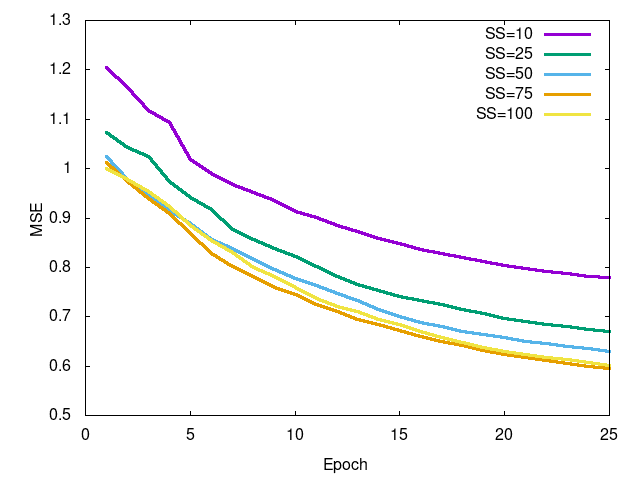
\includegraphics[scale=0.60]{images/pso-ss-plot.png}
\caption{Collected results for PSO-NN Swarm Size test}
\label{fig:pso-nn-ss}
\end{figure}

Performing an ANOVA test yields a $p$ value of $p < 0.0001$ and an F-score of $F = 8.45303$ which means the test is strongly confident in rejecting the null hypothesis: there is a measured benefit to using one or some parameter choices over the others.

Using Tukey's range test again by comparing means of pairwise samples, it is found that any pair involving a swarm size of $10$ has a significant difference of means.

To verify SS=10 is an outlier test, a second ANOVA test is performed using all samples excluding SS=10, yielding a $p$ value of $p = 0.167209$ and an F-score of $F = 1.72399$, meaning there is strong confidence in there being no significance in choosing a swarm size of $25$, $50$, $75$, or $100$.

Choosing a smaller swarm size linearly increases the speed of training as there are less particles to update positions upon. Even if the arithmetic operations used to move particles is relatively cheap, for such an expensive training mechanism, any decrease in training time is welcome.

\pagebreak

\subsection{PSO-NN Swarm Parameters Test}

The final test is to test a triplet of parameters controlling how particle swarms move during training. This tests yields the below plot:

\begin{figure}[h!]
\centering
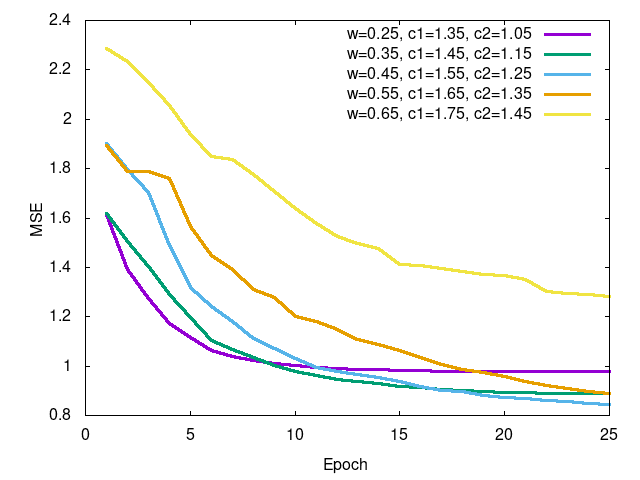
\includegraphics[scale=0.60]{images/pso-par-plot.png}
\caption{Collected results for PSO-NN Swarm Parameter test}
\label{fig:pso-nn-par}
\end{figure}

On performing an ANOVA test, a $p$ value of $p < 0.0001$ is found with an F-score of $F = 19.88014$ showing strong confidence that the null hypothesis should be rejected: there is significance in choosing some samples over others.

To verify, Tukey's range test is again used to compare pairwise means between samples and it is found the final parameter choice is an outlier with a much higher mean. To verify, removing this sample and running another ANOVA test shows no significance in choosing one sample over another, suggesting that any other parameter is appropriate.

These parameters are found through experimentation and there is no real guideline to choosing adequate particle swarm parameters. These parameter triplets were chosen after some trial-and-error.

The relationship between inertial weight and cognitive and social coefficients is difficult to discern. Increasing or decreasing one of these swarm parameters will have unpredictable effect on convergence as it is abstract how these parameters interact with each other and other network parameters such as hidden layer size and swarm size [1].

\subsection{Summary of Results}

On conclusion of tests, in many instances ideal parameters were found and in other instances results suggested any parameter is appropriate with the exception of one parameter outlier.

\begin{table}[h!]
\centering
\begin{tabular}{|c|c|c|}
\hline
\textbf{Hidden Layer Size} & \textbf{Learning Rate} & \textbf{Momentum Rate} \\ \hline
10 & 0.100 & 0.001 \\ \hline
\end{tabular}
\caption{Idealized BP-NN parameters}
\label{Tab:bp-nn-ideal}
\end{table}

\pagebreak

For backpropagation, the hidden layer size was found to be sufficient at $10$, $15$, and $20$ neurons with no statistical advantage of one over another. However, since the hidden layer size is directly related to the speed of training and speed of convergences, a smaller value is better. Therefore a hidden layer size of $10$ neurons is chosen.

For learning rate, only one parameter choice was appropriate: a learning rate of $0.100$. Lower learning rates converged slower or not at all, and the tested higher learning rate failed to converge completely.

Lastly, for momentum rate, any parameter choice between $0.001$, $0.010$, and $0.100$ can be chosen as there is very little correlation between momentum rate and speed of training. Any difference in execution speed results in a minute number of extra arithmetic operations which do not significantly hamper performance. To this end, a momentum rate of $0.001$ is chosen.

\begin{table}[h!]
\centering
\begin{tabular}{|c|c|c|}
\hline
\textbf{Hidden Layer Size} & \textbf{Swarm Size} & \textbf{Swarm Parameters} \\ \hline
5 & 25 & $\omega = 0.45, c_1 = 1.55, c_2 = 1.25$ \\ \hline
\end{tabular}
\caption{Idealized PSO-NN parameters}
\label{Tab:pso-nn-ideal}
\end{table}

For particle swarm training, the hidden layer size test showed significance in choosing five neurons in its hidden layer over the other options as it converged quicker and offered the fastest training time. While the confidence in this test was beyond the point of absolute reliability, it was not as confident as other tests. Nevertheless, there is clear advantage to using a smaller hidden layer for this training method.

In testing swarm size, only the smallest swarm size of ten was determined to be an outlier case and any other swarm size was adequate in training the network. To this end, a swarm size of $25$ is chosen as it was the next smallest swarm size tested, and swarm size is directly correlated to speed of training.

Lastly, swarm parameters were examined and it was found that an inertial weight of $0.65$, cognitive coefficient of $1.75$ and social coefficient of $1.45$ was inappropriate for training. Any other set of swarm parameters was adequate in training the network.

\subsection{Performance}

MSE is the measure in which a network is tested. MSE is inversely related to classification error and therefore a lower MSE means better classification.

\begin{figure}[h!]
\centering
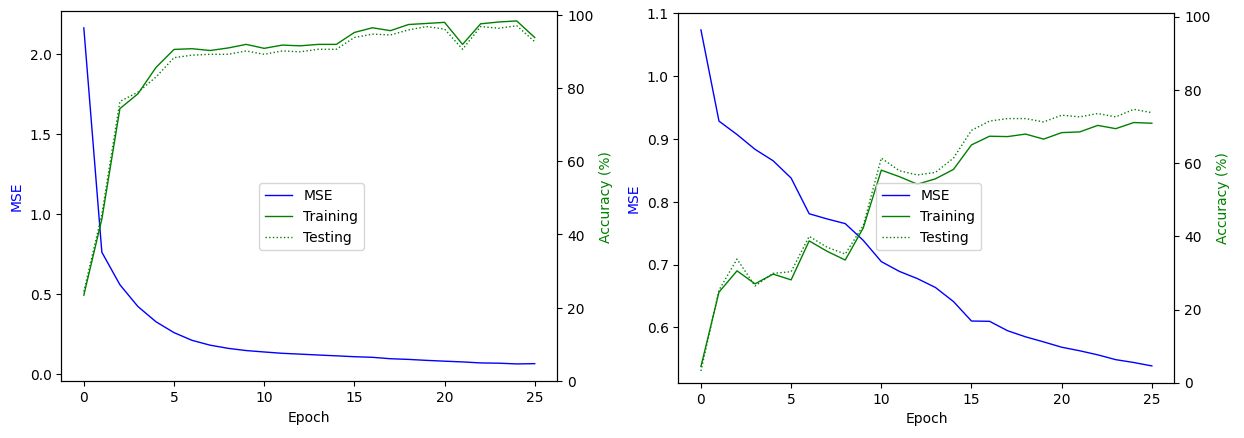
\includegraphics[scale=0.48]{images/compare.png}
\caption{Comparison of sample runs of BP-NN and PSO-NN}
\label{fig:plot-compare}
\end{figure}

\pagebreak

In the above figure, a single execution of BP-NN and PSO-NN training is performed using the idealized parameters. In these plots, the MSE and accuracy against the training and testing data sets is plotted versus epochs.

Of immediate note is BP-NN is able to converge much quicker and to a smaller MSE. The termination conditions is MSE $\leq 0.2$, which typically reflects in a network accuracy of 95\%+.

Unfortunately, PSO-NN is unable to meet this target within $25$ epochs and instead is able to reach approximately 70\% accuracy. However, considering a random guess at classification is only 11\%, the performance is still promising.

Between the two network types, BP-NN outclasses PSO-NN in convergence speech, reaching the termination condition, and speed of training.

\section{Conclusion}

On comparing backpropagation to particle swarms in training a neural network, differences arise in architecture as well as idealized hyperparameters. Oftentimes they are opposing, such as hidden layer size suffering from being small in backpropagation but flourishing for particle swarms.

Using metaheuristics to train networks is advantageous when the problem space is not linearly differentiable. Gradient based techniques for training networks also suffer from many pitfalls due to the error gradient, such as exploding or vanishing gradients.

However, metaheuristics like particle swarm optimization are more suited for smaller problem sizes and recognizing thermopile sensor data for classification is a relatively difficult problem with large dimensionality.

Backpropagation excels at most problem sizes as evidenced in this report and the parameter choices are very lenient with every test converging better than any given particle swarm test---even if some of those parameters are not ideal. This strengthens the idea of backpropagation being a good "go-to" approach for training a network when other methods are more obtuse or difficult to implement.

By analyzing parameter choices for backpropagation and particle swarms, a good baseline on training parameters was found to at the very least perform better than random guessing, whether using a gradient based or metaheuristic based approach to training.

\section{References}

\noindent [1] Gudise, et al., \textit{Comparison of Particle Swarm Optimization and Backpropagation as Training Algorithms for Neural Networks} [\textit{2003 IEEE Swarm Intelligence Symposium}] 2003.

\vspace{3mm}

\noindent [2] K. Mehrotra, et al, \textit{Elements of Artificial Neural Networks}. MITPress, Cambridge, Massachusetts, 1996.

\vspace{3mm}

\noindent [3] T. M. Mitchell, \textit{Machine Learning}. McGraw-Hill, New York, 1997.

\vspace{3mm}

\noindent [4] N. Qian, \textit{On the momentum term in gradient descent learning algorithms} [\textit{Neural Networks, vol. 12, no. 1, pp.145-151}]. Online, 1999.

\vspace{3mm}

\noindent [5] Patrick K. Simpson, \textit{Artificial Neural Systems: Foundations, Paradigms, Applications, and Implementations}. Elsevier Science Inc., 1996.

\end{document}
